%% grundlagen.tex
%% $Id: grundlagen.tex 28 2007-01-18 16:31:32Z bless $
%%

\chapter{Basics \& Related Work}
\label{ch:Basics}

\section{Schlafmedizin}
\label{ch:Basics:se:schlafmedizin}
% start seite 3-5 im buch schlafmedizin_1x1 
Unter dem Begriff \textit{Schlafmedizin} versteht man die Lehre von Diagnostik, Klassifikation und Behandlung von Störungen währrend des Schlafs \cite{schlafmedizin_1x1}. 
Trotz Erwähnungen in der Antike findet Schlafmedizin erst seit des letzten Jahrhunderts Bedeutung.
Mithilfe der Polysomnographie konnten unterschiedliche Schlafphasen zyklischen Ablaufs erkannt werden.
Zudem konnten den Schlafphasen physiologische Eigenschaften nachgewiesen werden.
Heutzutage sind ca. 80 Schlafstörungen in dieversen Bereichen bekannt, welche neben psychologischen Testverfahren überwiegend elektrophysiologisch untersucht und behandelt werden.
Patienten werden mit ambulanten Hilfsmitteln oder stationär in einem Schlaflabor untersucht und anschließend von einem technisch ausgebildeten Personal analysiert.

Hierbei wird eine Polysomnographie durchgeführt, womit genauere Messergebnisse im Vergleich zu einem ambulanten Hilfsmittel (z.B eine Langzeitbewegungsmessung), erreicht werden können.
Währrend einer Polysomnographie werden Gehirnströme, Augenbewegungen und Muskelspannungen erkannt, wodurch die einzelnen Schlafphasen unterschieden werden können.
Die verschiedene Sensorwerte werden dann in Form eines Hypnogramms mittels der Kriterien des AASM (engl. \textit{American Association for Sleep Medicine}) ausgewertet (siehe \ref{hypnogram_example}). 
Hierbei werden die Schlafstadien in \textit{Wachphase (w)}, \textit{Einschlafen (N1)}, \textit{leichten Schlaf (N2)}, \textit{Tiefschlaf (N3)} und \textit{Rapid-Eye-Movement-Schlaf (REM)} unterteilt.

\begin{figure}[ht]
    \centering
    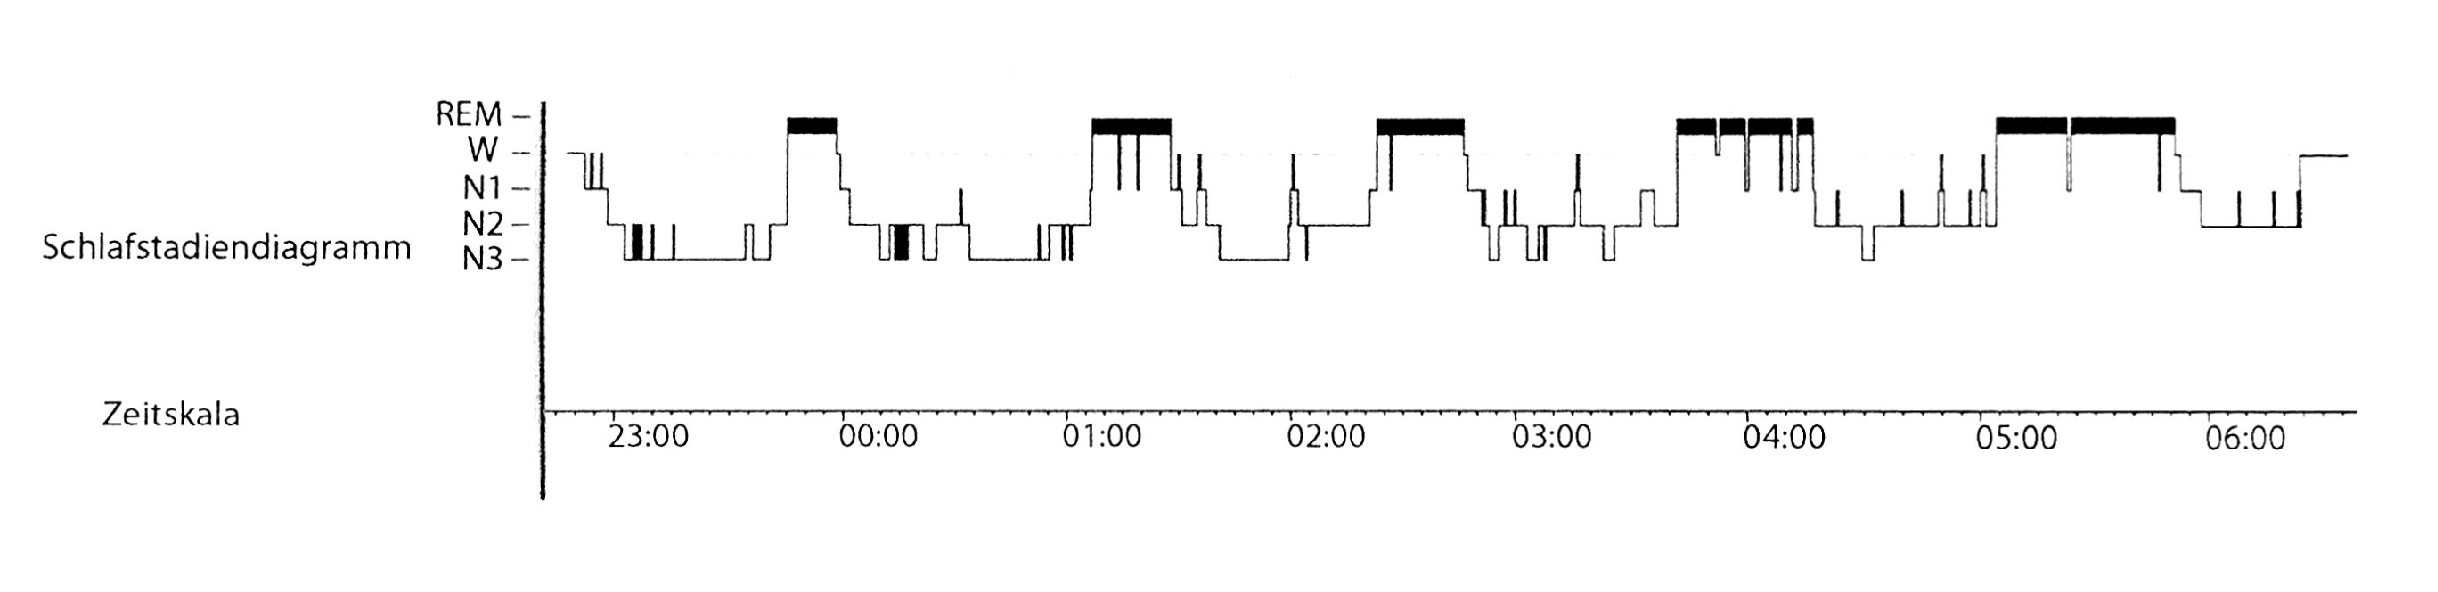
\includegraphics[scale=0.33]{respiration/hypnogram_example}
    \caption{Beispielaufzeichnung, dargestellt in einem Hypnogramm \cite{praxis_der_schlafmedizin}}
    \label{hypnogram_example}
\end{figure}

% ende cite
% start seite 9- im buch schlafmedizin_1x1 
Im Schlaflabor werden zudem auch Untersuchungen der Müdigkeit, der Tagesschläfrigkeit und der Aufmerksamkeit vorgenommen \cite{schlafmedizin_1x1}.

Atmungsstörungen können oft die Ursache von Schlaganfällen, Herzinfarkten oder den eben genannten Symptomen sein, welche zu erheblichen psychischen Störungen führen können.
% ende cite
Aus diesem Grund ist es wichtig, so genau wie möglich Schlafstörungen bestimmen zu können, um Folgeerkrankungen zu verhindern. 

\section{Klassifizierung von Schlafstörungen}
Zur Charakterisierung von Schlafstörungen werden viele Biosignale währrend des Schlafs registriert, welche entscheidene Merkmale liefern \cite{praxis_der_schlafmedizin}.
Aufgrund dieser Annahme wurden Klassifikatoren für Schlafstörungen entwickelt.
\begin{itemize}
    \item Ein- und Durchschlafstörungen (Insomnien)
    \item Schlafbezogene Atmungsstörungen
    \item Hypersomnien zentralnervösen Ursprungs
    \item Zirkadiane Rhythmusschlafwachstörungen
    \item Störungen in Verbindung mit Schlaf, Schlafstadien oder partiellem Erwachen (Parasomnien)
    \item Schlafbezogene Be wegungsstörungen
    \item Andere Schlafstörungen
\end{itemize}

Diese Gliederung orientiert sich an der \textit{ICSD-3} \cite{praxis_der_schlafmedizin}.


Diese Bachelorarbeit fokussiert sich darauf, ein zentrales Schlafapnoe zu klassifizieren, was Bestandteil der {\glqq schlafbezogenen Atmungsstörungen\grqq} ist.
Schlafapnoe wird in obstruktives und zentrales Apnoe unterschieden. 
20\% aller Erwachsenen haben 5 oder mehr obstruktive Ereignisse pro Schlafstunde \cite{schlafmedizin_1x1}.
Zentrales Apnoe hingegen tritt seltener auf, als obstruktives Apnoe, jedoch auffällig oft bei besonderen Patientengruppen. 
Ein Beispiel liefern Patienten mit Herzinsuffizien und einer eingeschränkten kardialen Pumpfunktion.
72\% dieser Patientengruppe leidet unter zentralem Schlafapnoe. Dies stellt die Bedeutung der Klassifikation deutlich klar, da eine genaue Erkennung eines zentralen Apnoes hier sehr wichtig ist.

\subsection{Zentrales Schlafapnoe}
Beim zentralen Apnoe steht der Luftfluss trotz offener Atemwege für mindestens $10\si{\s}$ still. Dies kann vollständig (zentrales Apnoe), oder partiell (zentrales Hypopnoe) erfolgen. 
Ab einer Anzahl von 5 Apnoeereignissen wird zentrales Apnoe diagnostiziert.
Die Ursachen gelten hierbei internistischer oder neurologischer Grundlage.
Typische an- und abschwellige Muster sind durch eine chronische Herzinsuffizienz, durch eine verlängerte Kreislaufzeit, oder durch eine zentralnervöse Verstellung der sogenannten Apnoeschwelle zurückzuführen.
Der $CO_2$ Gehalt im Blut wird als Apnoeschwelle bezeichnet.
Am Tag sind die Symptome von zentralem Apnoe eher an deren Ursache, den internistischen und neurologischen Grunderkrankungen zu erkennen, da diese häufig nicht von den Symptomen der Schlafapnoe zu unterscheiden sind. 
In der Nacht wird zentrales Apnoe, ebenso wie obstruktives Apnoe an Atemaussetzern, häufig vom Partner des Patienten beobachtet.
Zudem kann lautes und unregelmäßiges Schnarchen ein Indiz für ein Apnoe sein, ebenso wie ein Aufwachen in Atemnot.

Ein Schlafapnoe kann jedoch in unterschiedlichen Schweregraden auftreten. 
Es gibt Patienten, welche kaum bis keine Probleme haben und nur aufgrund von nächtlichen Erkenntnissen ihrer Ehepartner zum Arzt geschickt werden. 
Es gibt jedoch auch Patienten, die am Tag Probleme haben, bei monotonen Situationen wach zu bleiben.

Eine Diagnose würde mögliche Folgeerkrankungen schneller erkennbar machen und die Ursache dieser erklären.

\section{Maschinelle Lernverfahren}
Zur Klassifikation eines zentralen Apnoes werden im Rahmen dieser Bachelorarbeit verschiedene Klassifikationsverfahren verwendet, wobei Trainingsdaten gesammelt werden, welche dann zentrale Apnoeereignisse anhand dieser Trainingsdaten klassifizieren sollen.

Maschinelle Lernverfahren sind Algorithmen, welche die Performance des Algorithmus mittels Trainingsdaten verbessern \ref{add ref} \todo{reference Maschine Learning course of KIT}. 
Es wird zwischen folgenden Lernverfahren unterschieden:
\begin{itemize}
    \item Supervised Learning
    \item Unsupervised Learning
    \item Reinforcement Learning
\end{itemize}
Beim \textit{Supervised Learning} sind die Trainingsdaten im Vergleich zum \textit{Unsupervised Learning} markiert. 
So wird beim \textit{Supervised Learning} anhand von markierten Trainingsdaten eine Entscheidung getroffen. 
Anhand der folgenden Tabelle wird bei \textit{Supervised} und \textit{Unsupervised Learning} zwischen verschiedenen Modellen unterschieden:
\begin{center}
    \begin{tabular}{ | l | l | }
      \hline
      \textbf{Supervised Learning} & \textbf{Unsupervised Learning} \\ \hline
      \hline
      Regression & Clustering \\ \hline
      Klassifikation & Dimensionsreduktion \\
      \hline
    \end{tabular}
\end{center}

Jeder Algorithmus, welcher in einem Maschinellen Lernverfahren eingesetzt ist, besteht aus 3 Teilen: Zum einen der \textit{Representation}, der \textit{Evaluation} und der \textit{Optimization}. 
In der \textit{Representation} unterscheidet man nach dem zugrunde liegenden Modell, welches beispielsweise ein Entscheidungsbaum, ein neuronales Netz oder eine Support-Vektor-Maschine sein kann.
Die \textit{Evaluation} behandelt die Frage, in welche Richtung die Entscheidung getroffen werden soll. 
Ein Beispiel hierfür wäre die Genauigkeit, den Precision \& Recall, die Entropie oder den Likelihood-Schätzer.
Beim dritte Teil, der \textit{Optimization}, wird eine Optimierung des Algorithmus angestrebt. 
Dies kann unter anderem mit Methoden 2. Ordnung, Zufälliger Suche, einem absteigenden Gradienten oder der Methode der kleinsten Quadrate versucht werden.

Das in dieser Bachelorarbeit verwendete Lernverfahren ist \textit{Supervised Learning} mit dem zugehörigen Modell, die \textit{Klassifikation}.
Zur Evaluation wurden verschiedene Klassifkationsverfahren verwendet, welche im Folgenden genauer erläutert werden.

\subsection{Random Forest}
\todo{wie funktioniert das?}

\subsection{XGBoost}
\todo{wie funktioniert das?}

\subsection{SVM}
\todo{wie funktioniert das?}


\section{Forschung von Klassifikation anhand von IMU-Daten}
Es gibt bereits Ansätze, welche sich damit befassen, Alternativen zur Ermittlung von Schlafstörungen zu finden. 
Somit könnte ein Besuch im Schlaflabor durch einen bequemen Test ersetzt werden. 
Ein vielversprechender Ansatz ist es, mittels IMU-Daten die Bewegung des Körpers zu messen und anhand dieser Informationen die Atmung oder ähnliches herauszufiltern, um dann Rückschlüsse auf Schlafstörungen schließen zu können.

\subsection{Accelerometer am Brustkorb}
Bereits 2018 gab es Forschung in diesem Bereich. \textit{Phan Duy Hung} hat sich damit befasst, einen Accelerometer an den Brustkorb zu fixieren \cite{hung_central_2018}.
Es wurde versucht, durch die Platzierung an genau dieser Stelle das Herzschlagen genauer erkennen zu können. 
Die Rohdaten zeigen hierbei bereits die Herzfrequenz und die Atmung des Probanden (siehe Abb. \ref{imu_research_hung_rawData}).

\begin{figure}[ht]
    \centering
    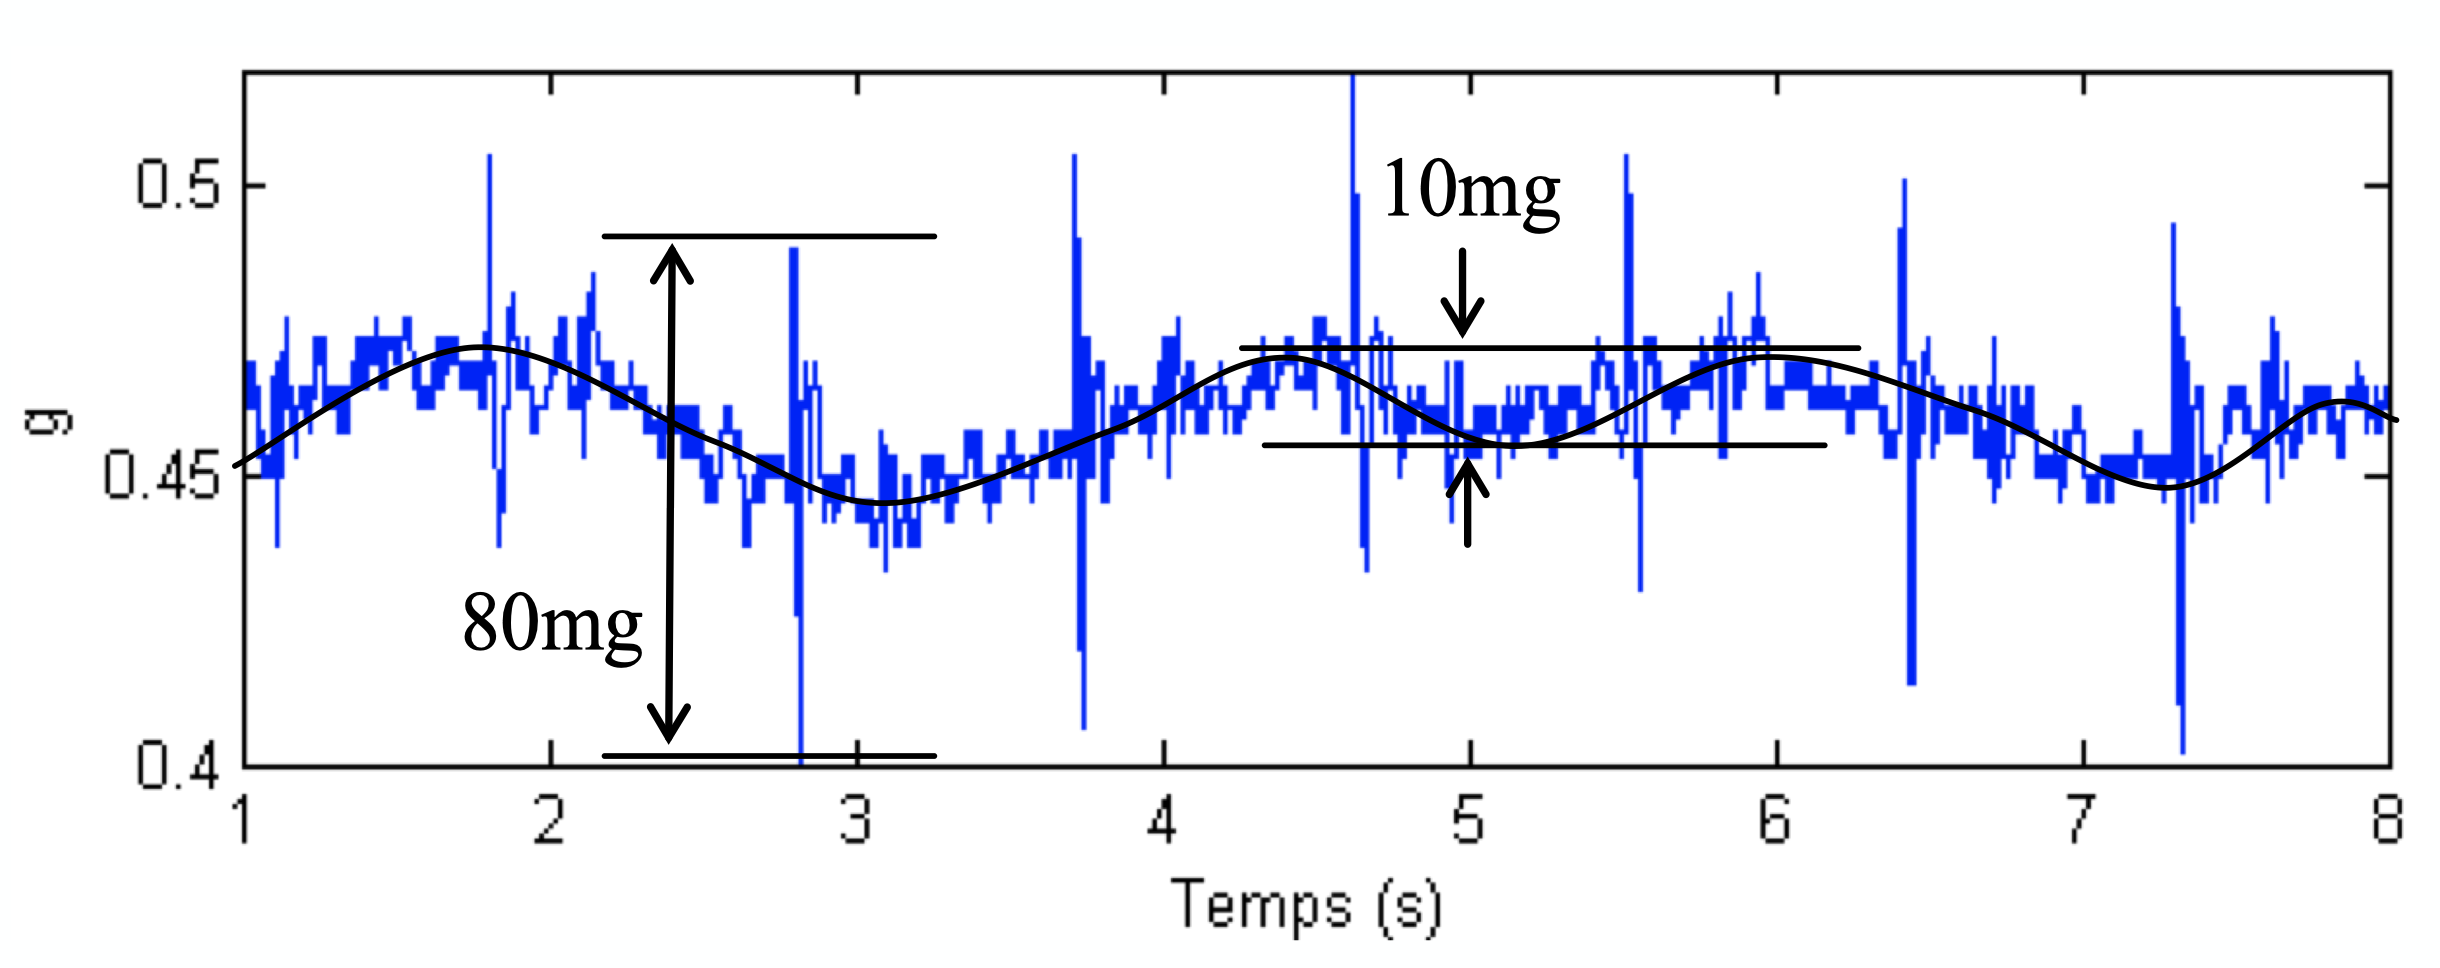
\includegraphics[width=1\textwidth]{imu_research/Paper_Hung_rawData}
    \caption{Rohdaten des Accelerometers in \cite{hung_central_2018}}
    \label{imu_research_hung_rawData}
\end{figure}

Die Daten wurden nach der Aufzeichnung durch einen Bandpassfilter mit adaptiver Apassung optimiert, um die SNR (\textit{signal-noise-ratio}) zu verringern.
Der Puls wurde ermittelt, indem Peaks (Max: \textit{V}-Peak, Min: \textit{R}-Peak) gefunden und als Herzschlag interpretiert wurden.
Des weiteren musste Signalrauschen, z.B von der Reibung des T-Shirts und Haut, aus dem Signal herausgefiltert werden. 
Zudem wurden 3 Features anhand der Amplitude über die Zeit berechnet. 
Das erste Feature ist die \textit{Spektralverhältnis (spectral ratio)}. 
Hier wird ein Leistungsspektrum einminütigems Segments vom HR-Signal geschätzt. 
Der Frequenzbreich zwischen [0-1] $\si{\hertz}$ wurde untersucht. 
Dieser Bereich spiegelt die Frequenzvariation zwischen zentraler Schlafapnoe und normaler Aktivität wieder.

Im Bereich von [0,3-0,6] Hz zeigt sich das Maxima der spektralen Leistung, was immer in der Größenordnung abnimmt. 
Dieser Wert wird normiert, indem er durch den Mittelwert der spektralen Leistung im Bereich [0,1-0,3] Hz geteilt wird. 
Das Verhältnis der max(P) im Bereich von [0,3-0,6] Hz zum Mittelwert(P) in [0,1-0,3] Hz ist unabhängig von der Person.

Das zweite Feature sind die \textit{Wavelet- Koeffizienten (wavelet coefficients)}, bei welcher die Analyse mit mehreren Auflösungen und guter Lokalisierungsfähigkeit im Zeit-Frequenz-Bereich häufig eine Wavelet-Transformation verwendet wird. 
Hierbei wurde das Atemsignal in 5 Ebenen mit der db2-Wavelet zerlegt. Danach wurden die Standardabweichungen der Detailkoeffizienten in den Ebenen 4 und 5 verwendet. 

Das dritte Feature sind die \textit{linear prediction coefficients}. 
Die zweite Ordnung der linearen Vorhersage
\begin{center}
    $x(n) = a_1 x(n-1) + a_2 x(n-2) + e(n)$
\end{center} 
wurde verwendet, wobei x eine Zeitreihe ist, e(n) der Vorhersagefehler und {a1, a2} die Vorhersagekoeffizienten, die durch die Least-Square-Optimierungsverfahren zu bestimmen sind.

Die folgenden Werte wurde zum Testen mit ANOVA ausgewählt: \\
ANOVA: $a_1$, $a_2$ und $\sqrt{a_1^{2} + a_2^{2}}$


Zudem wurden nichtlineare Features in Betracht gezogen, da bereits vorher festgestellt wurde, dass in komplexen Atemuntersuchungen lineare Funktionen nicht ausreichen. Die Herzfrequenz wird hierbei als Timeseries betrachtet.
Es wurden diesbezüglich die nichtfunktionalen Features der \textit{Poincaré-Plots (Poincare plot geometry)}, \textit{Trendbereinigende Fluktuationsanalyse (Detrended Fluctuation Analysis)}, \textit{Approximate-Entropie (Approximate Entropy)}, sowie der \textit{Ljapunow-Exponent (Largest Lyapunov exponent)} verarbeitet. 

Die Features wurden anschließend mit der \textit{ANOVA-Toolbox} ausgewertet.
Somit konnte ermittelt werden, ob in dem zeitlichen Intervall ein Apnoe stattgefunden hat, oder nicht.

Durch dieses Paper wurde eine Genauigkeit von 84.2\% erreicht, ein zentrales Apnoe zu erkennen und mit 84.1\% konnte ermittelt werden, dass in diesem Zeitrahmen kein zentrales Apnoe vorkam.


\subsection{Detektion direkt am Kopf mittels der Google Glass Brille}
2015 wurde erforscht, durch Informationen des Google Glass den Puls und das Atemsignal zu ermitteln \cite{hernandez_cardiac_nodate}. 
Der Vorteil hierbei ist die Position der Brille. 
Da sie Am Kopf platziert ist, liefert die Brille möglicherweise vielversprechende Werte im Vergleich zu IMU-Daten, die am Brustkorb aufgezeichnet worden sind.
Die Google Glass wurde allerdings nicht entwickelt, um physiologische Daten zu sammeln, kann jedoch dafür verwendet werden, da alle nötigen Sensoren (Accelerometer, Gyroscope und Kamera) verbaut hat.
Die Resultate liefern einen mittleren absoluten Fehler (\textit{MAE}) von 0.82 Schlägen pro Minute (STD: 1.98) der Herzrate und 0.6 Atmungen pro Minute (STD: 1.19) bei der Atmung unter Betrachtung verschiedener Beobachtungsfenster und Kombinationen der Sensoren. 
\begin{figure}[ht]
    \centering
    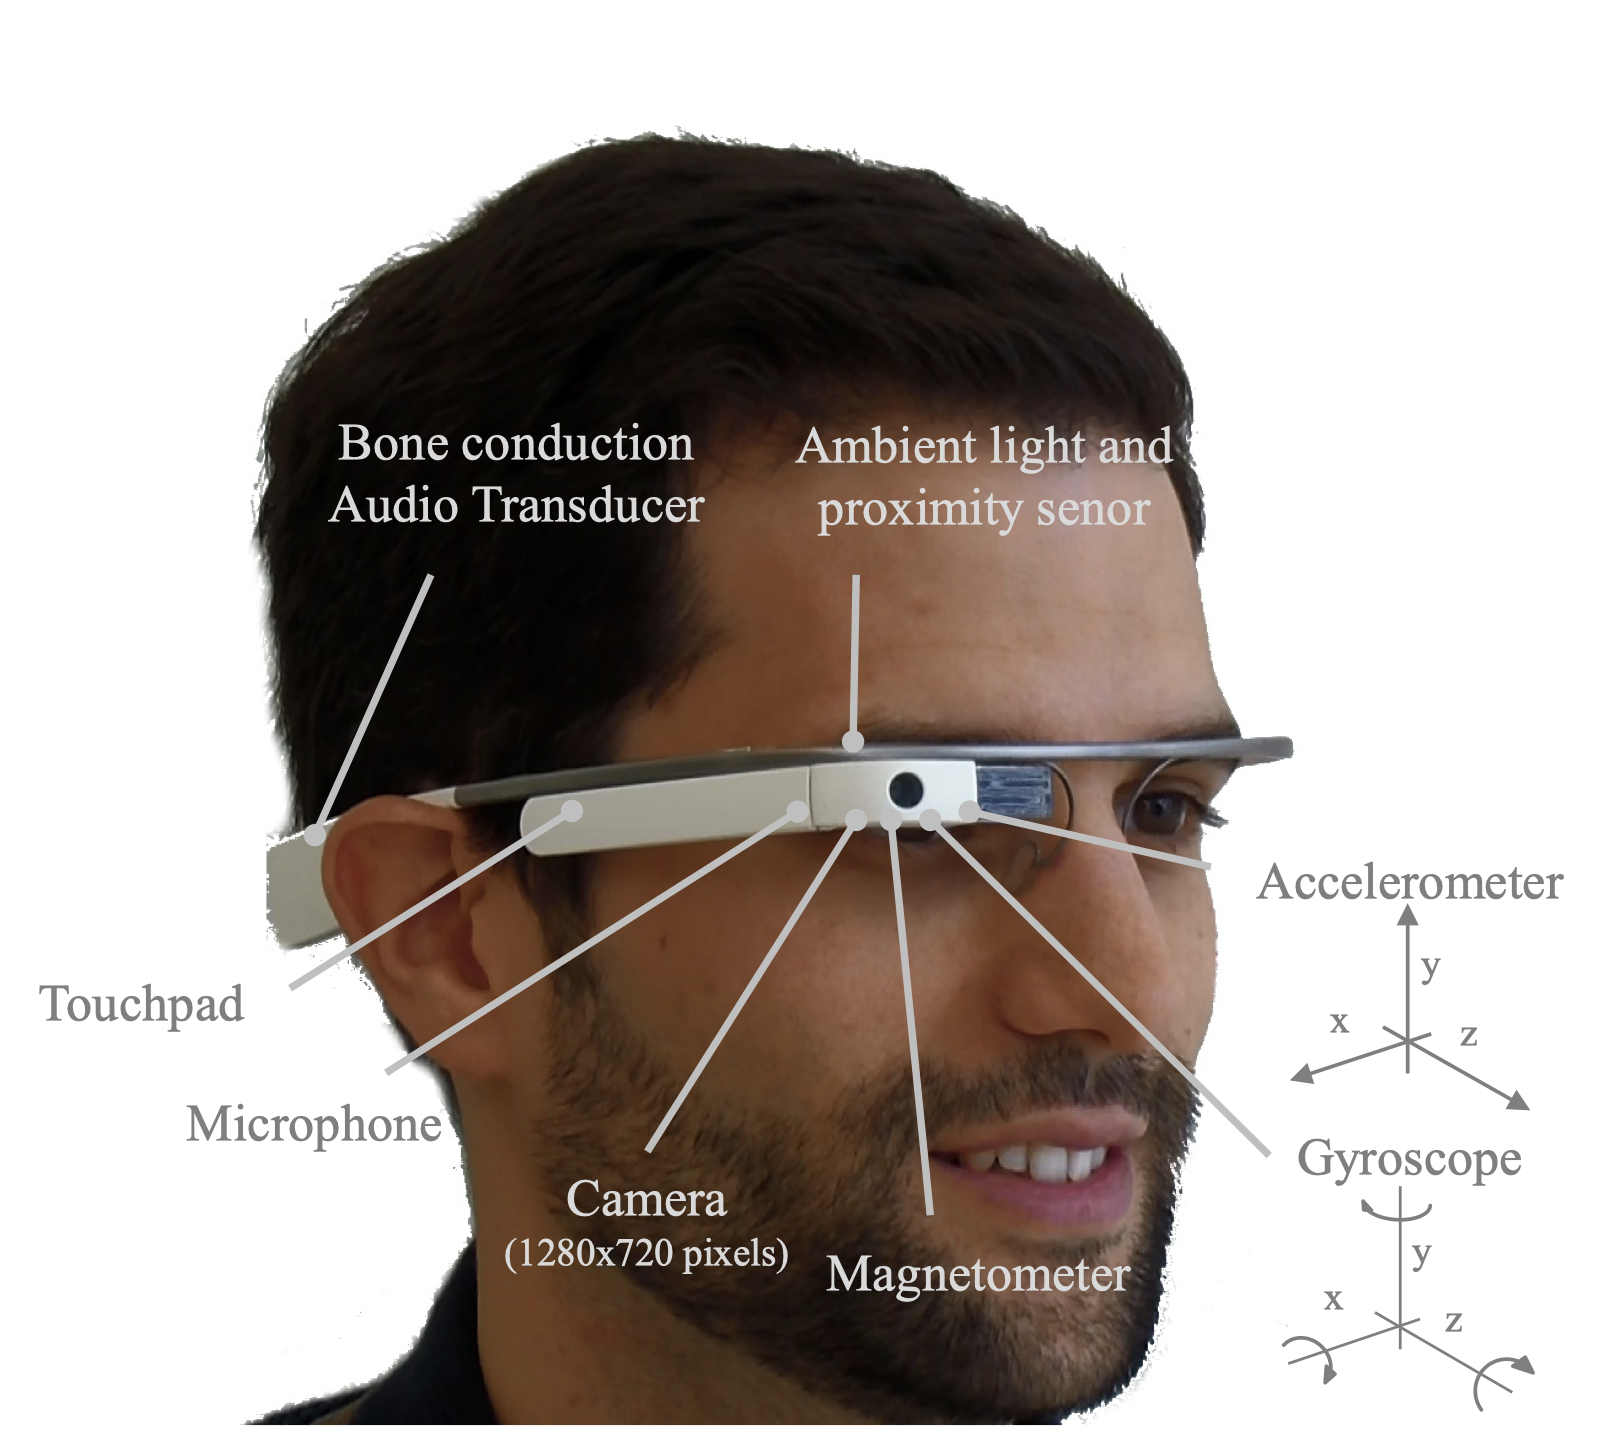
\includegraphics[width=\textwidth / 2]{imu_research/googleGlass}
    \caption{Google Glass Sensordaten \cite{hernandez_cardiac_nodate}}
    \label{imu_research_google_glass}
\end{figure}
Die Herausforderung lag zudem daran, stromsparende Echtzeitberechnungen mit Algorithmen zu entwickeln, womit physiologische Parameter extrahiert werden. Der Nutzer soll das Gerät im Alltag normal weiternutzen können. 

Es wurden 2 Techniken entwickelt, eine zur Ermittlung des Pulssignals und die andere für das Atemsignal.
\subsubsection{Pulssignal}
Die Schätzung des Pulssignals wurde anhand einer Timeseries von Vektoren in mehrere Schritte aufgeteilt:
\begin{itemize}
    \item Von jeder Dimension des Vektors wurde ein gleitendes Durchschnittsfenster von 3 Abtastwerten subtrahiert, wodurch Signalverschiebungen und Trends entfernt werden konnten.
    \item Ein Bandpass Butterworthfilter der 4. Ordnung mit Cut-Off Frequenzen von $10 \si{\hertz}$ und $13 \si{\hertz}$ wurde auf jede Dimension angewendet, um Veränderungen des BCG zu isolieren
    \item Zudem wurde ein Bandpass Butterworthfilter der 2. Ordnung mit den Cut-Off Frequenzen von $0.75 \si{\hertz}$ und $2.5 \si{\hertz}$ (entspricht 45 and 150 Schläge die Minute) angewand, was schließlich das resultierende Pulssignal liefert.
\end{itemize}

\begin{figure}[ht]
    \centering
    \begin{subfigure}{.49\textwidth}
        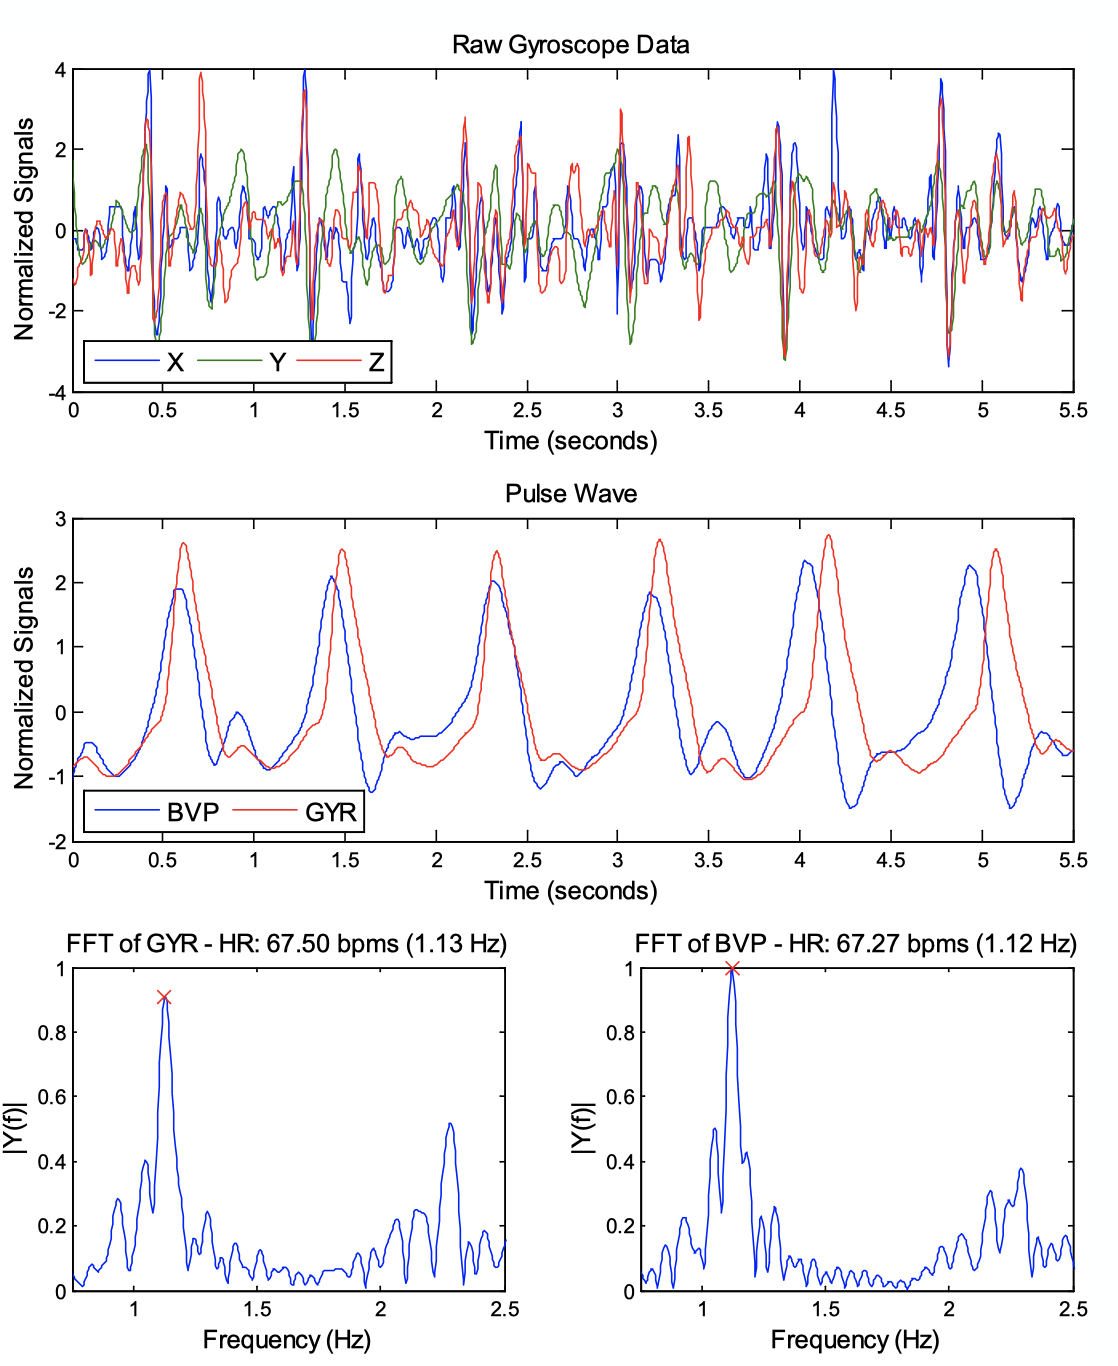
\includegraphics[width=\textwidth]{imu_research/googleGlass_pulse_fig2}
      \caption{Beispiel eines Pulssignals mittels der Gyroskopdaten (rot) und des Ground-Truth Signals (blau). Die beiden unteren Graphen zeigen das Fouriespektrum von jedem Signal (FFT: Fourier Spectrum, GYR: Gyroscope, BVP: Blood Volume Pulse, HR: Heart Rate, bpms: beats per minute)}
      \label{background:googleGlass:pulse_wave}
    \end{subfigure}
    \begin{subfigure}{.49\textwidth}
        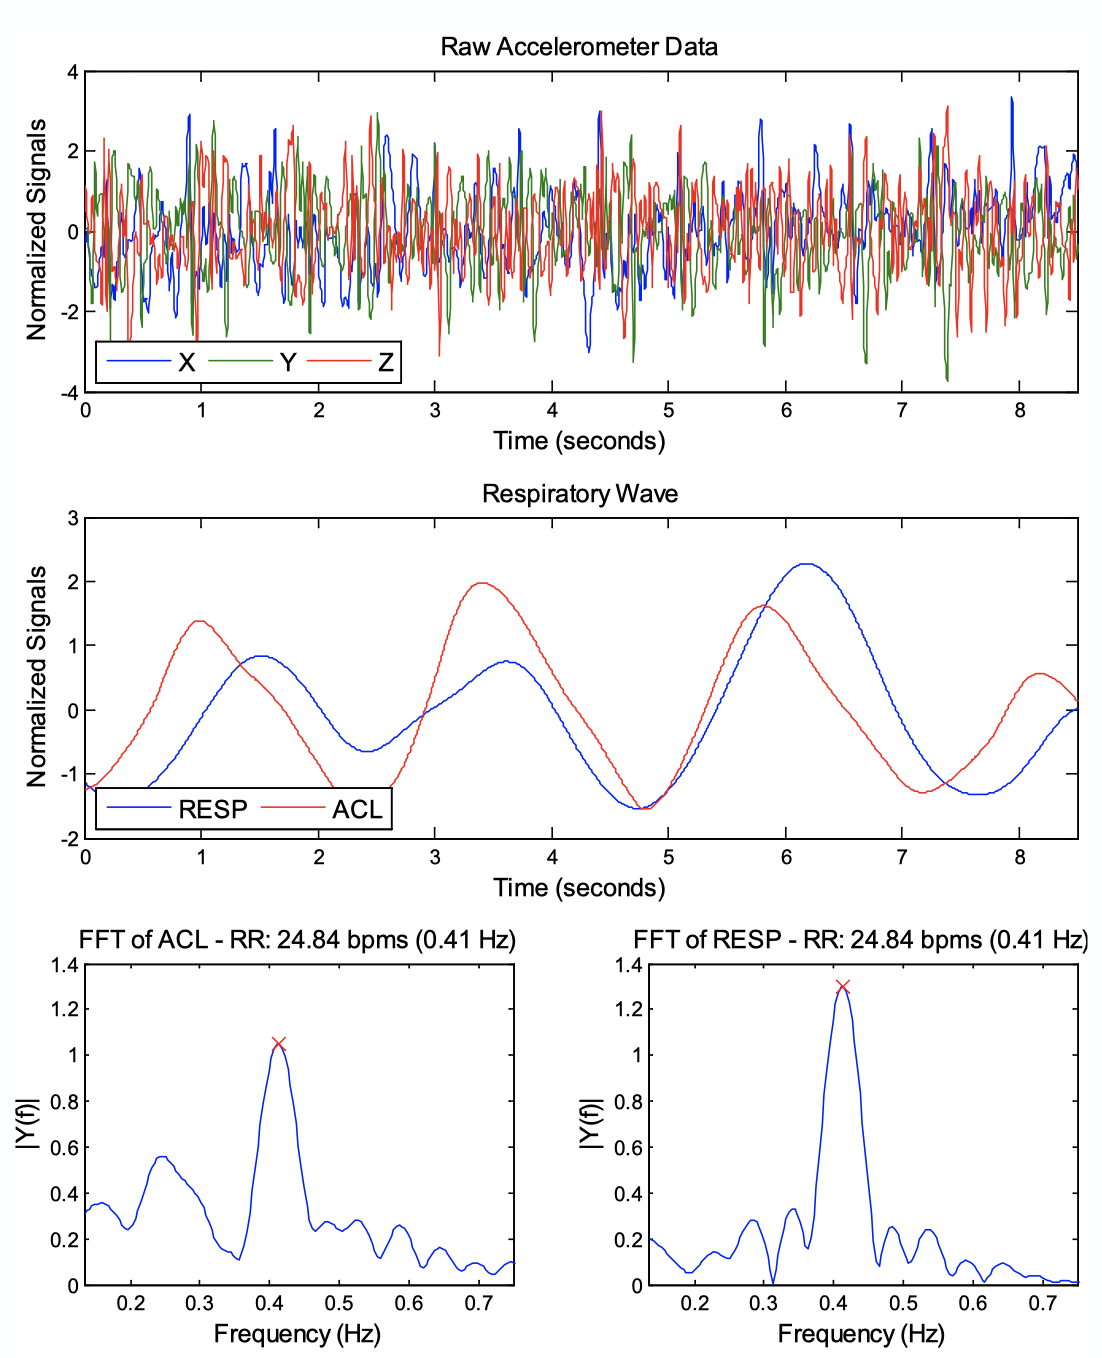
\includegraphics[width=\textwidth]{imu_research/googleGlass_respiratory_fig3}
      \caption{Beispiel einer Schätzung des Atemsignals anhand der Beschleunigungsdaten (blau) und des Ground-Truthsignals (rot). Die beiden unteren Graphen zeigen das Fourierspektrum von jedem Signal. (FFT: Fourier Spectrum, ACL: accelerometer, RESP: Respiration from chest band, RR: respiration rate, bpms: breaths per minute)}
      \label{background:googleGlass:respiratory_wave}
    \end{subfigure}
    \caption{Herzrate- und Atemfrequenzanalyse}
    \label{background:googleGlass}
  \end{figure}

Die Abbildung \ref{background:googleGlass:pulse_wave} zeigt ein Signal des Herzschlags, gesammelt von den Informationen der Gyroskopdaten. Diese Daten wurden von dem Google Glass aufgezeichnet, währrend der Person auf dem Rück lag. Der obige Graph zeit ein 3-Achsen Gyroskop signal über eine Dauer von 5.5 Sekunden. Der mittlere Graph zeigt die Schätzung des Herzschlags, nachdem die vorgestellten Methoden angewandt wurden in rot, die des Referenzsignals in blau. Es ist sehr gut zu erkennen, dass die Schätzung sehr nahe an den Referenzsignalen ist.

\subsubsection{Atemsignal}
Das Atemsignal wurde durch verschiedene Schritte berechnet:
\begin{itemize}
    \item Ein gleitender Mittelwertfilter wurde auf jede Komponente angewandt. Die Fensterlänge wurde auf die Dauer eines Atemzyklus gesetz, in diesem Fall 45 Atmungen pro Minute. 
    \item Ein Bandpass Butterworthfilter der 4. Ordnung mit dem Cut-Off Frequenzen von $0.13 \si{\hertz}$ und $0.75 \si{\hertz}$ (entspricht 8-45 Atmungen pro Minute) wurde auf jede Dimension angewandt.
    \item Da die verschiedenen Dimensionen der Sensoren nicht in Relation zu den Körperpositionen stehen, wurde eine Principal Component Analyse angewandt, um einen derartigen Einfluss zu reduzieren. Nach einer Fast Foiuriertransformation (FFT) auf jede Komponente wurde das Signal mit der Periode mit der maximalen Größenordnung ausgewählt, welche innerhalb des betrachteten Frequenzbereichs liegt.
\end{itemize}

Die Abbildung \ref{background:googleGlass:respiratory_wave} zeigt ein Beispiel einer Atemfrequenzschätzung der Beschleunigungsdaten eines Patienten. Wie zu sehen ist, sind die Daten sehr nahe an dem Referenzwert, welcher mit aufgezeichnet wurde.


\subsection{Überwachung von Puls und Atmung mittels eSense-Earpods}
2019 wurde von \textit{Tobias Röddiger}, \textit{Daniel Wolffram} und \textit{David Laubenstein} nachgewiesen, dass es möglich ist, mittels den eSense-Earpods die Atmung und den Puls näherungsweise zu ermitteln \cite{roddiger_towards_2019}. 
Dies gelang etwas genauer, als das Monitoring von \textit{J. Hernandez} mit dem Google Glass \cite{hernandez_cardiac_nodate}
Es wurden hierbei eine Studie mit 12 Personen aufgezeichnet, welche in 3 Positionen (liegend, stehend, sitzend) jeweils vor, bzw. nach einer sportlichen Bewegungsphase einen einminütigen Atemablauf durchgeführt haben. 
Die Analyse der Daten erfolgte im Anschluss der Studie und wurde in einer Pipeline verarbeitet, welche zuerst das Rauschen reduziert, anschließend einen Triangle-Filter der Breite $2\si{\s}$ anwendet und danach eine PCA (engl. \textit{principal component analysis}) ausführt, um die Daten unabhängig von deren Achse zu bewerten.
Nun wurden Windows mit der Größe von $20\si{\s}$ extrahiert, welche die die Atmung und den Puls anhand dieses Windows berechnen.
Die Resultate ergaben einen mittleren absoluten Fehler (engl. \textit{mean absolute error}) von 2.62 CPM (acc) und 2.55 CPM (gyro), jedoch variieren diese von Proband zu Proband.

\todo{extend with more content from this paper}

\begin{figure}[ht]
    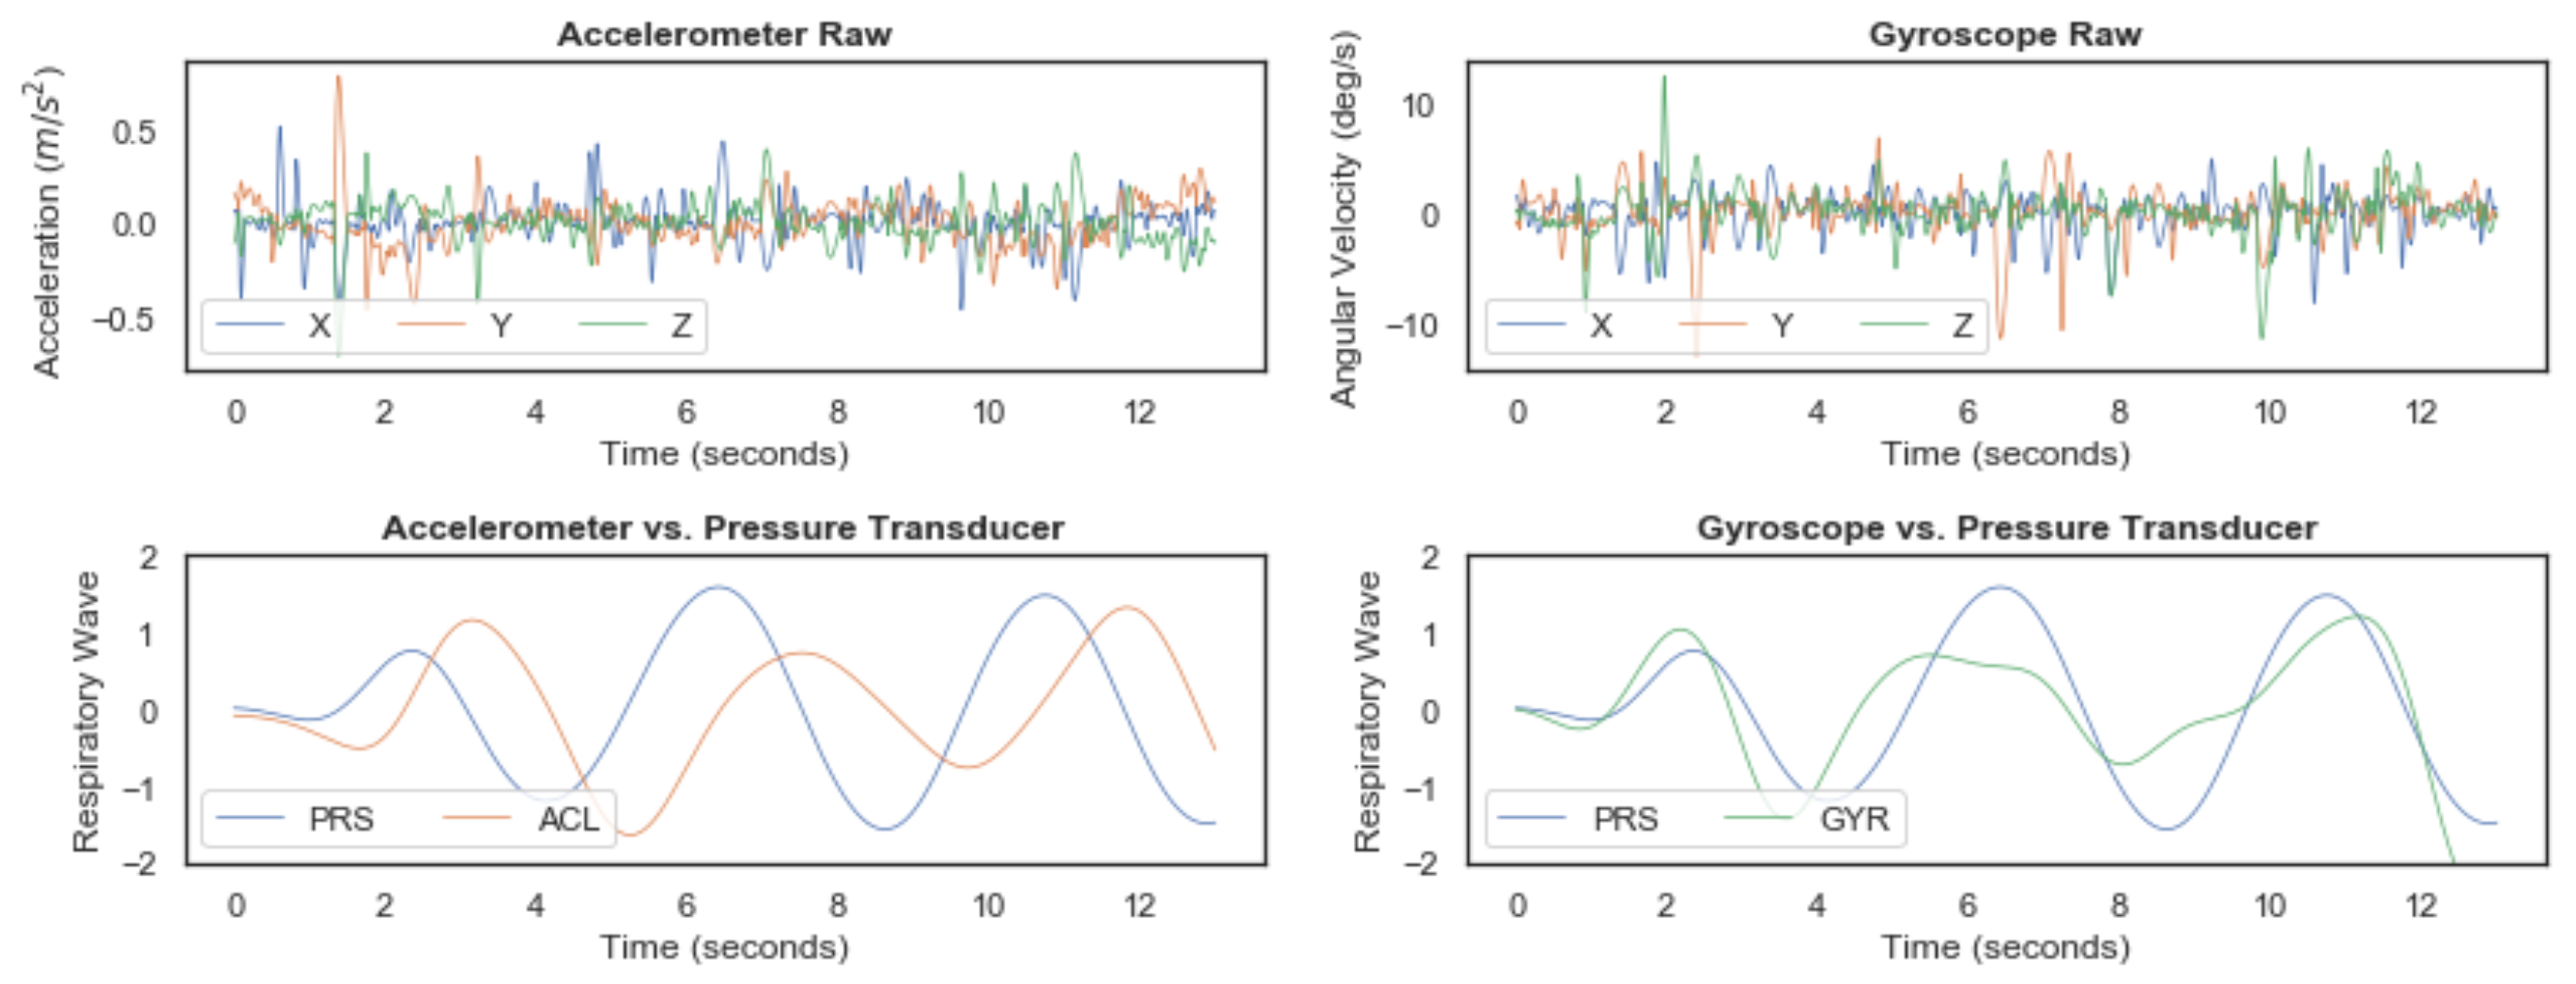
\includegraphics[width=1\textwidth]{imu_research/towards_resp_rates_waves}
    \caption{Rohdaten der Accelerometer und Gyroscope daten innerhalb von $12 \si{\s}$, sowie die Atem- und Pulsschätzung, verglichen mit dem Ground-Truh (blau)}
    \label{background:towards_resp_esense:results}
\end{figure}